\documentclass{article}
\usepackage{amsthm,amsfonts}
\usepackage{graphicx}

\input{pat.tex}
\newcommand{\cn}{\mathsf{cr}}
\newcommand{\dn}{\mathsf{dn}}

\begin{document}

\begin{thm}
For any outerplanar graph $G$, $\dn(G)\le 3$.
\end{thm}

\begin{proof}
Without loss of generality, we may assume that $G$ is maximal
outerplanar.  We call each cycle of length 3 in $G$ a triangle of $G$.
An embedding of $G$ using only three edge lengths is obtained as
follows:  Select any triangle of $G$ as the \emph{root triangle}.
Embed the root triangle's vertices at the points $p_0=(0,0)$,
$p_1=(1,0)$ and some point $p_2=(x,y)\in[0,1]\times[0,1]$ whose
coordinates will be specified later.  The root triangle shares an edge
with up to three other triangles of $G$.  Embed each of these by
reflecting the root triangle through the line supporting the common
edge of the two triangles.  Repeat this process recursively to embed
all the triangles of $G$.

We will show that there is a choice of the point $p_2$ for which the
given embedding is a drawing of $G$ by showing that, for any vertex
edge pair $(v_i,e_j)$ the set of choices of $p_2$ for which the
embedding of $v_i$ is contained in the embedding of $e_j$ is a
1-dimensional set.  Thus, the set of choices of $p_2$ for which some
vertex lies on some edge is a finite union of 1-dimensional sets.
However, $p_2$ can be selected in to be any point in
$[0,1]\times[0,1]$, a 2-dimensional set, so it suffices to select any
$p_2$ that is not in any of the 1-dimensional sets.

Note that, by a change of coordinates, we may assume that $e_j$ is an
edge of the root triangle.  We distinguish between two cases.  In the
first case, $e_j$ is the segment $[p_0,p_1]$, i.e., the bottom edge of
the root triangle.  Let $f:[0,1]\times[0,1]\mapsto \mathbb{R}^2$ be
the function that defines the location of $v_i$ given the location of
$p_2$.  The codomain (range) of $f$ is a 2-dimensional set and the
intersection of the segment $[p_0,p_1]$ with this set is a
1-dimensional set. The preimage of $[p_0,p_1]$ in $f$ is a
1-dimensional set.\notice{Justify these last two statements.} 

Next we consider the case where $e_j$ is one of the other two edges of
the root triangle, say the segment $[p_0,p_2]$.  In this case,
consider the representation of $p_2$ using polar coordinates
$(\ell,\theta)$ where $\ell=\|p_0p_2\|$ and $\theta=\angle p_1p_0p_2$.
By a change of coordinates, we may assume that the segment $[p_0,p_2]$
is contained in the $x$-axis so that the root triangle has vertices
$p_0=(0,0)$, $p_2=(-\ell,0)$ and $p_1=(-\cos\theta,\sin\theta)$.
Again, the parameters $\ell$ and $\theta$ can be selected from a
2-dimensional set and there is a function $g$ that defines the
location of $v_i$ given $\ell$ and $\theta$.  However, the crucial
point to note is that, if the image of $v_i$ is contained in the
segment $[p_0,p_2]$ then it is on the $x$ axis.  The preimage of the
$x$-axis in $g$ is a 1-dimensional set in the parameter space
$(\ell,\theta)$ which is also a 1-dimensional set in the parameter
space $(x,y)$, as required.\notice{Justify the second last statement}
\end{proof}

Note that, without some further ideas, it is not possible to
generalize the above proof to show that $\dn(G)\le 2$ if $G$ is
outerplanar.  In particular, with only two distance classes, all
triangles of $G$ are isosceles triangles defined by a single parameter
$\alpha$ that measures the angle at the apex.  In this case, the range
of the function $g$ is a 1-dimensional set and this set can coincide
with the line containing $[p_0,p_2]$.  The example in the figure below
shows an example where this occurs.  In this example, any choice
of $\alpha$ in the interval $[0,\pi/6]$ results in the vertex $v_i$ being
embedded on the segment $[p_0,p_2]$.

\begin{tabular}{cccc}
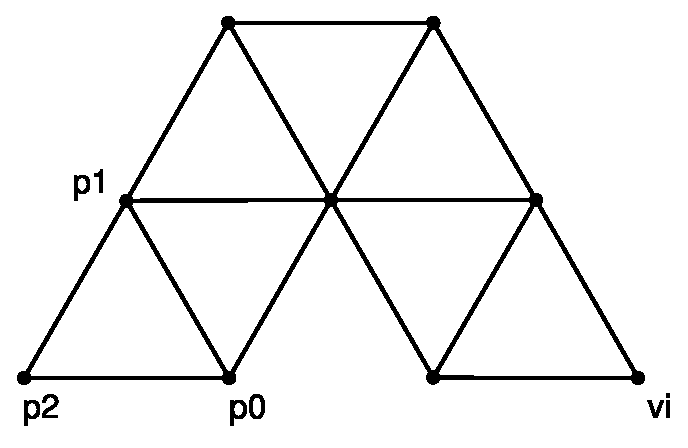
\includegraphics[scale=.30]{no2-1} &
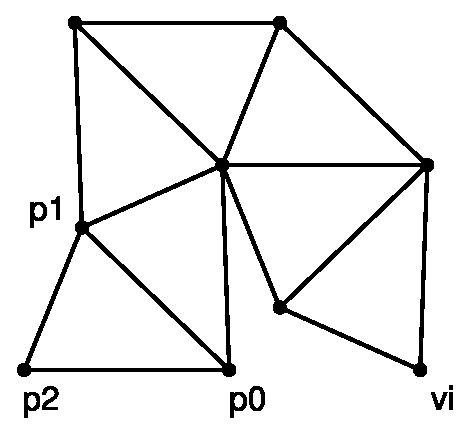
\includegraphics[scale=.30]{no2-2} &
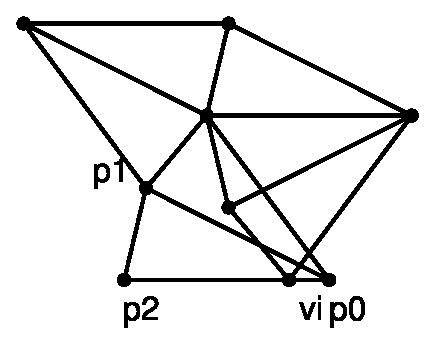
\includegraphics[scale=.30]{no2-3} &
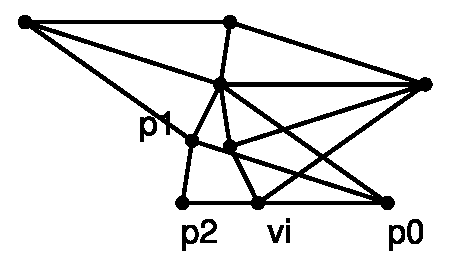
\includegraphics[scale=.30]{no2-4} 
\end{tabular}

\end{document}
